\begin{figure*}[!t]
\centering
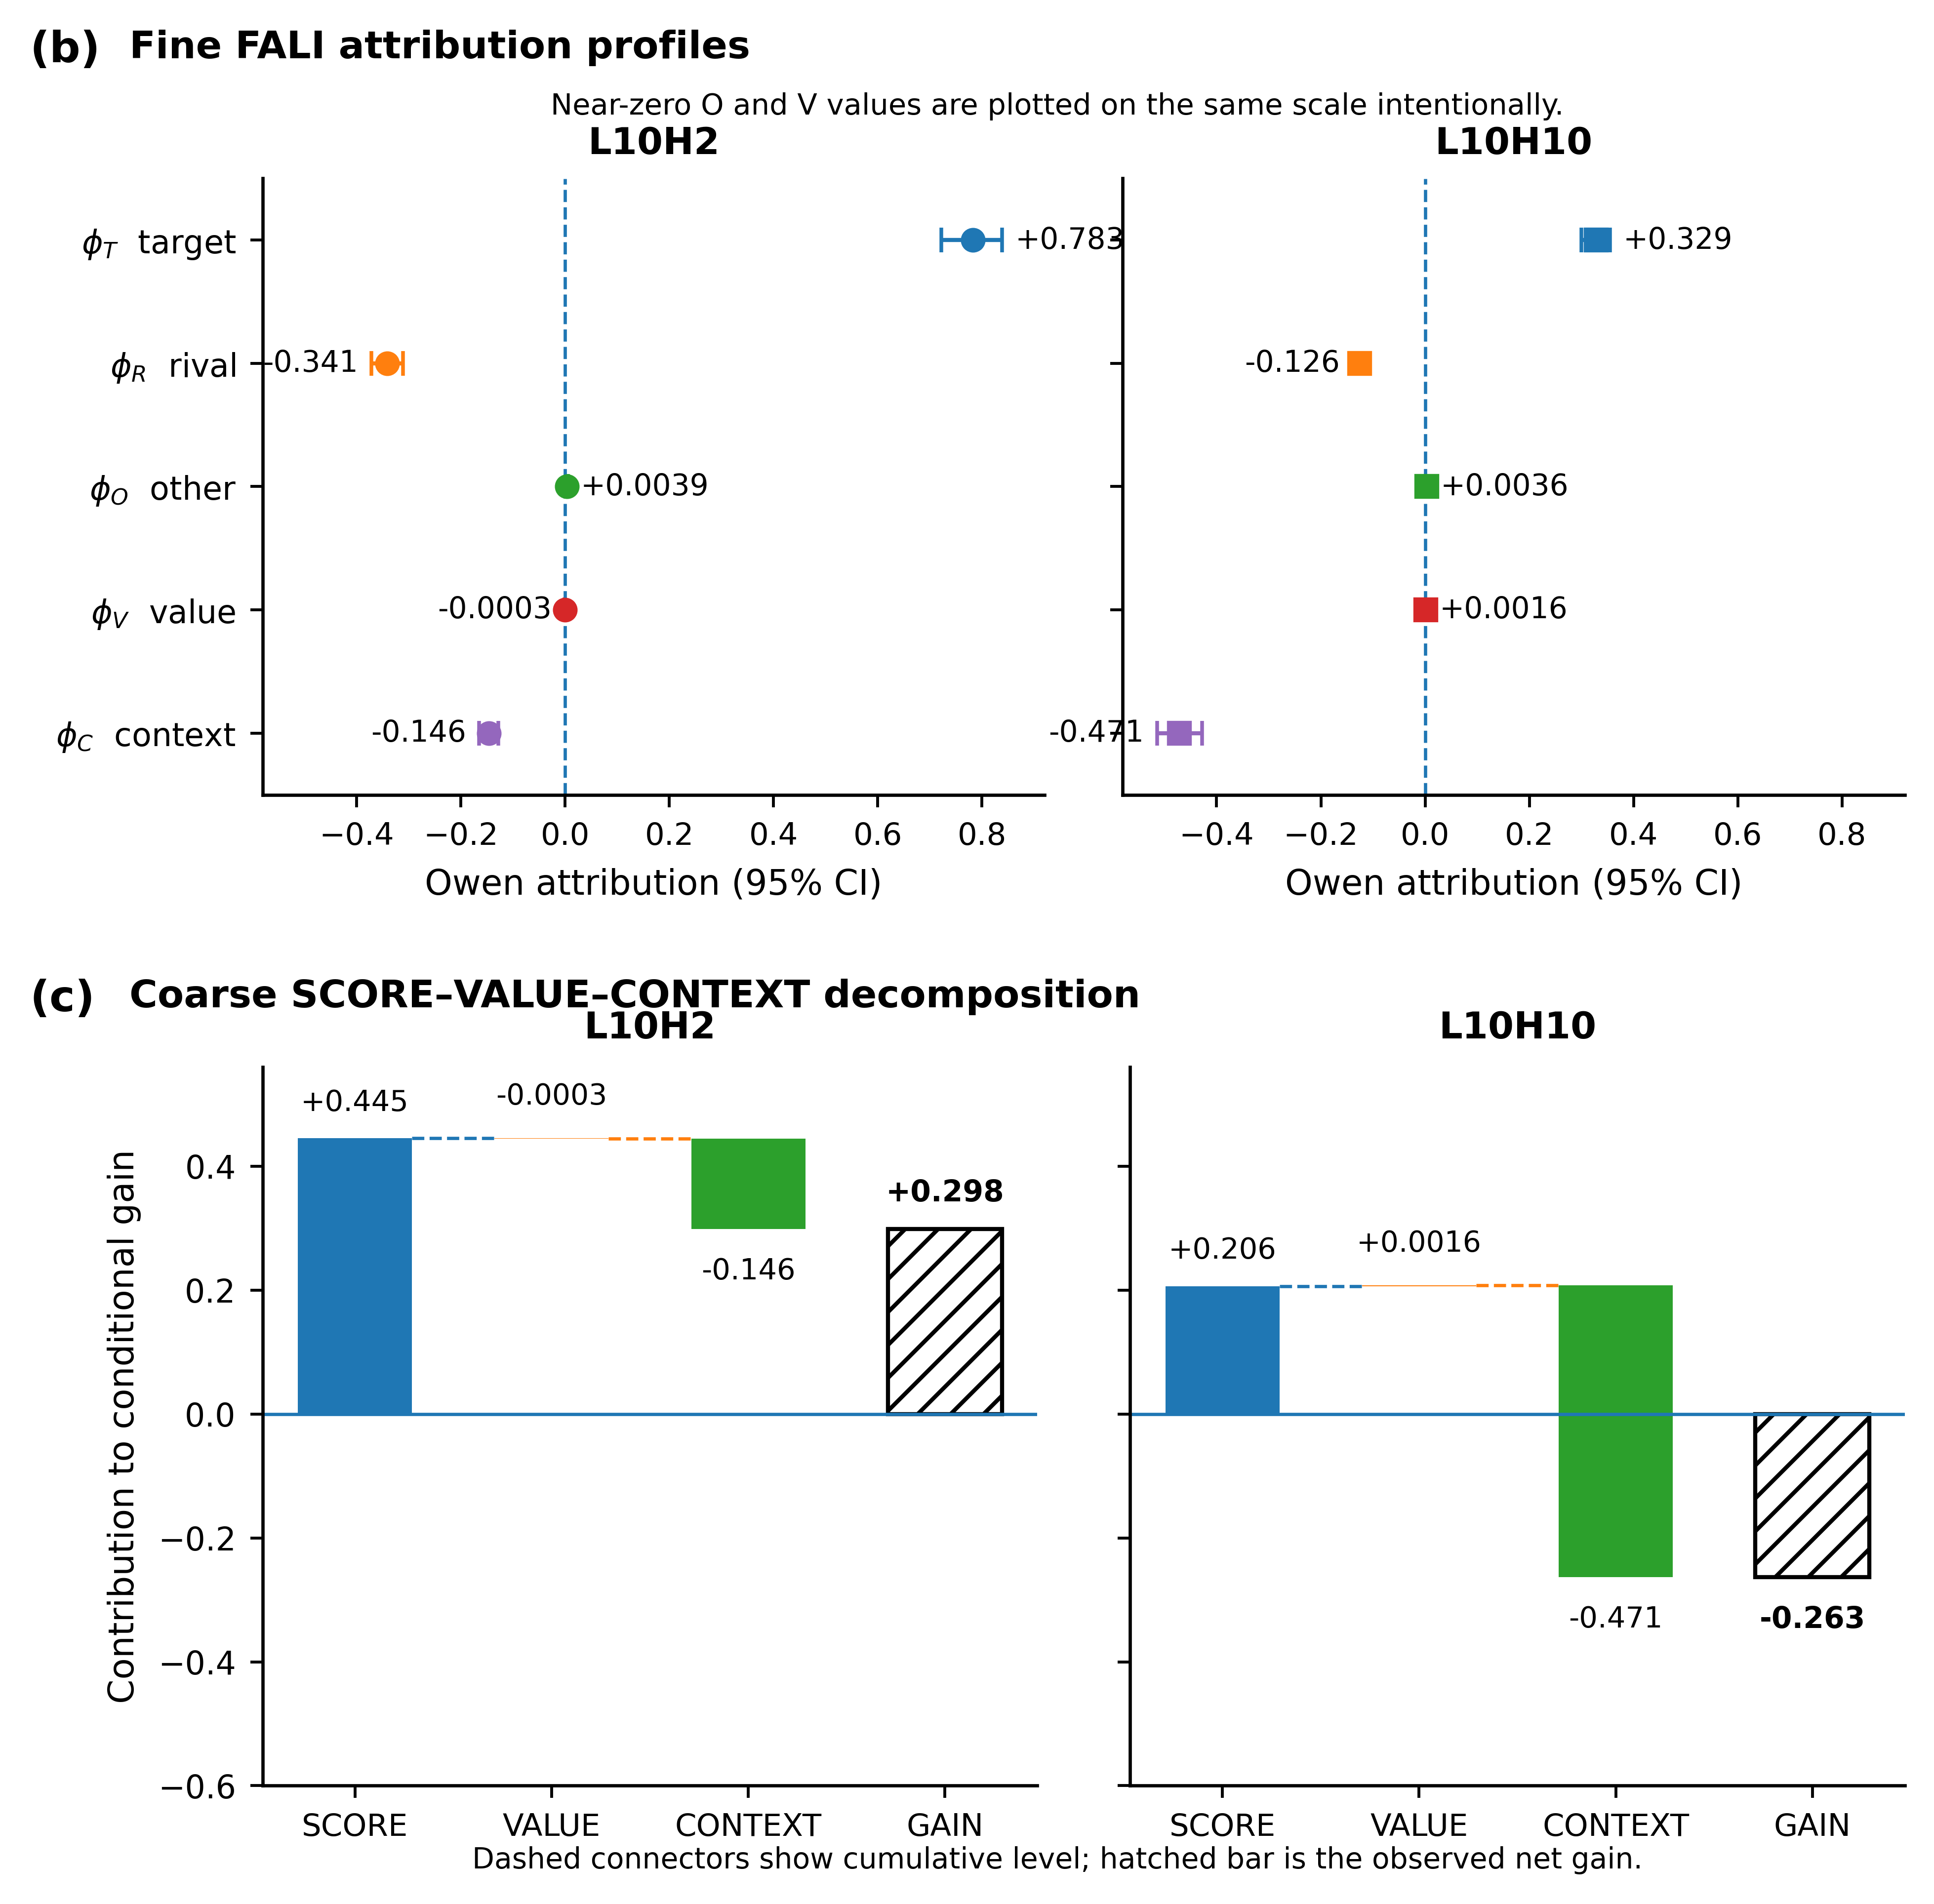
\includegraphics[width=0.92\textwidth]{figures/Fig4bc.png}
\par\smallskip
\noindent\textbf{Figure 4 (continued).} Fine and coarse FALI decomposition in GPT-2 IOI.
(b) Both L10H2 and L10H10 have positive target-score and negative rival-score contributions under the canonical FALI game; $O$ and $V$ remain near zero on the same plotted attribution scale.
(c) The coarse SCORE/VALUE/CONTEXT decomposition explains why the same fine-score sign pattern does not imply the same functional response: L10H10 retains a positive SCORE contribution, but a substantially negative surrounding-context contribution outweighs it and produces a negative conditional gain.
Points are exact balanced means; intervals in panel (b) are hierarchical 95\% bootstrap confidence intervals. The context factor $C$ denotes surrounding-network/context contribution under the specified intervention game and is not a uniquely localized downstream mechanism.
\end{figure*}
